\chapter{Background}

Thanks to a dense protective atmosphere, Earth can withstand impacts from dust to boulder-sized objects traveling faster than bullets without so much as a dent on Earth's surface.
Many of these near-Earth objects are extremely small and don't leave much of a trace, but larger objects can leave a trail of light visible from Earth's surface as they burn up in our atmosphere.
In this chapter, we will discuss the classification of near-Earth objects, how fireballs are observed, and give important insight as to why and how we will compare our photometric survey with others.


\section{Description of Fireballs}

When considering types of near-Earth objects, many names come to mind: asteroids, meteors, meteorites, and fireballs are all often used interchangeably. 
However, there are several key distinctions between these objects.  
Traveling through space, asteroids are the largest of this group and are generally over \SI{10}{\meter} in diameter \cite{steel_meteoroid_1996}. 
These objects are responsible for massive craters that are visibly present on the Moon.
Meteoroids are anywhere between \SI{10}{\micro\meter} and \SI{10}{\meter} and are far more numerous than their asteroid cousins.  

Meteoroids or asteroids that pass through Earth's atmosphere become meteors.
As a meteor passes through our atmosphere, it begins to ablate.
Ablation begins when a fast moving meteor, typically traveling over \SI{10}{\meter/\second}, encounters air particles that slow it down.
This loss of kinetic energy is turned into heat and is hot enough to vaporize outer layers of the meteor.  
Atoms within these vaporized outer layers and nearby air molecules get energetically excited and then release light as they relax back to their natural state.
The amount of light that reaches an observer on Earth's surface can be measured in terms of apparent magnitude.
Magnitude is represented on an inverse $\log_{10}$ scale where dimmer objects are represented by high numbers and brighter objects are lower, and in many cases negative, values.
Magnitude is calculated as:

\begin{equation}
m = -2.5 \log_{10}(I/I_0)
\label{magnitude_equation}
\end{equation}

 
where $I$ is the intensity of the meteor/fireball and $I_0$ is the intensity of a reference brightness.  
Both intensity measurements are in units of $\si{\watt/\meter^2}$.
Meteors with an apparent magnitude below $-4$ qualify as bolides or fireballs.
For reference, in its brightest phase, Venus is a magnitude $-4.4$ planet while the dimmer Jupiter has a magnitude of $-2.1$ \cite{rao_venus_nodate}.
If an object is massive enough to withstand the heat of ablation in Earth's atmosphere and make it to the surface of Earth, it is classified as a meteorite. 
These are rare, occurring less than $200$ times per year.
Because meteorites are essentially rock remnants, they provide valuable information about the initial asteroid's origins.
While there is some overlap between asteroids, meteoroids, meteors, fireballs, and meteorites, their definitions are important to distinguish.
Figure~\ref{jed} graphically summarizes the relationship between these 5 terms.

\begin{figure}[ht!]
  \centering
  \includegraphics[scale=0.3]{images/jed_zoomedin.png}
  \caption[A depiction of near-Earth object classification.]{A depiction of near-Earth object classification.  Asteroids and meteoroids may be found in space, while meteors and their brighter counterparts, fireballs, burn up through Earth's atmosphere.  Unlike ordinary fireballs, meteorites remain intact and strike the surface of the Earth.}
  \label{jed}
\end{figure}

Our project specifically focuses on fireballs.
A fireball passing through the sky is referred to as a fireball event.
We may further classify fireball events into two categories: sporadic events and meteor shower events.
Meteor showers share an important relationship with comets.
Comets are celestial objects much larger than asteroids.
As comets travel through space, small bits of rock and ice separate from them.
This process is due to differences in pressures and heat on different areas of the comet.
Comet fragments make up a majority of the substance in meteor showers.


Meteor showers occur when Earth's orbit crosses paths with the orbit of a collection of debris. 
Such collections often orbit large masses such as Jupiter or the sun \cite{trigo-rodriguez_2006_2007}.
For example, the Perseid meteor shower has a highly elliptical orbit around the sun as seen in Figure~\ref{perceid}.  

\begin{figure}[ht!]
  \centering
  \includegraphics[scale=1.4]{images/persiod_shower.jpg}
  \caption[The Perseid meteor shower and its relation to our solar system.]{The Perseid meteor shower and its relation to our solar system.  Earth's orbit is shown in red (just inside of the yellow ring) while meteors in the shower are depicted as white dots.}
  \label{perceid}
\end{figure}

In contrast, there is debris in space that is not connected to any meteor shower. 
Events stemming from random debris are called sporadic events.
Debris in space can collect and becomes part of a larger system such as a meteor shower.
This is not the case for all space debris and is a direct result of unique gravitational circumstances.
Thus, sporadic events are less common.
Collecting information on fireball events allows astronomy researchers to develop a better understanding of the presence of matter in space. 

\section{Event Detection}

To compare our camera system to other professional systems, we must acquire enough event data to determine a flux rate.  
This section will discuss how different observation systems collect data on fireballs.
Particular emphasis will be placed on how the Willamette D6 Allsky Camera differs from professional cameras.


\subsection{Existing Surveys}
While amateur astronomers and low-budget systems can capture useful information, larger professional systems act as a vitally important comparison point.
Because many professional surveys are composed of multiple cameras working in unison, they have the advantage of multiple perspectives on a singular event.
This leads to more precise measurements of parameters like velocity, apparent magnitude, and location.
Individual events captured by an individual observer do contribute to the pursuit of knowledge.
However, a small camera system that cannot yield similar data to more professional surveys serves only a marginal amount of utility.

Cameras for Allsky Meteor Surveillance (CAMS), the SPanish Meteor Network (SPMN), NASA's Allsky Fireball Network and the LIncoln Near Earth Asteroid Research (LINEAR) program are examples of well-established existing meteor observing surveys.
All of these programs are continuously acquiring data and adding their findings to existing databases.  
Much of this data is widely available online, but varies from survey to survey.
% CAMS
Funded by NASA, Cameras for Allsky Meteor Surveillance (CAMS) aims to verify minor meteor showers and trace them back to their existing parent comets \cite{jenniskens_cams:_2011}.  
The project was created by Peter Jenniskens and is based in California.  
The CAMS network is spread across 3 different locations as seen in Figure~\ref{trio} and consists of over 60 cameras.
Each camera has a relatively narrow field of view of approximately \ang{30}.
When properly arranged, these cameras provide a high resolution image of the entire visible sky.
By spreading their cameras across three separate locations, the CAMS research group can measure precise trajectories of incoming meteors. 

\begin{figure}[ht!]
  \centering
  \includegraphics[scale=0.9]{images/CAMS_trio.jpg}
%   \setcaptioncitation{http://cams.seti.org/maps.html}
  \caption{The three CAMS network stations (yellow dots) within a 50 mile radius.}
  \label{trio}
\end{figure}



Similar to the phenomena of trying to catch a baseball with only one eye open, confidently capturing a three dimensional trajectory of a fireball is extremely difficult when using only one camera.
Multiple cameras provide different fireball-path perspectives and allow us to geometrically solve for the event's exact position.
Accurate trajectories are particularly useful in back-tracing the motion of the meteor's orbit.  
The CAMS team has reduced over $320,000$ of these orbits \cite{peter_jenniskens_cameras_2018}


%SPMN
The SPanish Meteor Network (SPMN) works in a similar fashion to the CAMS project.  
It consists of 25 observation stations located across Portugal and Spain \cite{trigo-rodriguez_2006_2007}.
In addition to becoming the first organization in Spain to successfully calculate the orbital path of a meteor, this organization revolutionized fireball research by developing the first CCD allsky cameras, or cameras that observe the entire visible sky \cite{jordi_l._pique_presentation_nodate}.
While this approach results in lower resolution event capturing compared to multi-camera systems, it is much cheaper and can cover the same sky area.
These cameras are now in use all across the world.

While SPMN and CAMS are powerful research organizations, their study of meteors only slightly overlaps with the research being discussed in this paper.
Because of their high grade equipment, they are able to capture data from extremely dim sources.
Fireballs, quantified by a magnitude below $-4$, compose only a small fraction of the meteors analyzed by these organizations.
Fortunately, other organizations focus specifically on larger and brighter events.

%Peter Brown
There are a multitude of ways that one can attain information about a fireball.  
All the aforementioned surveys have employed the use of photometric data.
In contrast, Peter Brown took data from the Department of Defense and the Department of Energy space-based systems in geostationary orbits.
The original purpose of these systems is to detect signatures of explosions near Earth's surface, but the system occasionally picks up false positives in the form of ablating bolides in the atmosphere.  
Because the system detects the amount of power released, Brown and others have used the systems to approximate a fireball's energy.
In a 2002 article published in \textit{Nature}, Brown estimated the optical energies of around 300 bolides.
His resulting flux rates are shown in Fig. \ref{brown} of the Introduction Section.
Drawing from this data set and other existing data sets, Brown compiled Equation~\ref{eq:browneq}, which relates bolide energy to the cumulative number of impacts on Earth each year. 

\begin{equation}
\log N = a_0 - b_0\log E
\label{eq:browneq}
\end{equation}
Here $N$ is the total number of objects colliding with Earth each year and $E$ is the respective energy of the sample in kilotons of TNT \cite{brown_p_flux_2002}.
In this empirically derived equation, $a_0 = 0.5677 \pm 0.015$ while $b_0 = 0.90 \pm 0.03$.
This relationship is known as a power law and will be a useful point of comparison for our Willamette D6 Allsky data.


%%%%%%%%%%%%%%%%%%%%%%%


\subsection{The D6 Allsky Camera}

% Overview
The Willamette University D6 Allsky Camera was created in 2016 to capture images of fireballs streaking through the night sky.
The aim of the project was to create an economically feasible and highly mobile observational system.
It is composed of a portable structure surrounding a monochrome security camera that is particularly light-sensitive.
The inside also host some necessary supporting devices, including a controlling Raspberry Pi. \cite{mcswain_using_2016}.
The assembly resembles a Star Wars astromech droid, and acquired its name from this inspiration.
The enclosure with visible camera is shown in Figure~\ref{droid}.
The D6 Allsky Camera is currently operational and has been gathering data since the summer of 2018.  
Below, we will discuss the design of the D6 Allsky Camera while also highlighting what makes it significant.

\begin{figure}[ht!]
  \centering
  \includegraphics[scale=0.7]{images/allsky_camera.png}
  \caption{The Willamette D6 Allsky Camera (2016). Paired with a little imagination it resembles an astromech droid from Star Wars.}
  \label{droid}
\end{figure}


% Components
The components of the D6 Allsky Camera are comprised primarily of 5 different pieces: the camera housing, a CCD camera, a thermostat and resistive heater, a video digitizer, and the Raspberry Pi to control everything.
The acrylic dome and PVC shell form the exterior of our system. 
The dome itself is a transparent half sphere that sits on top of a PVC cylinder that holds the system together.
Both act as a protective layer between the sensitive inside components and the outside environment.  
Without this feature, the system would be subject to rain, snow, dew, bug contamination, and other undesired effects.

The CCD camera is perhaps the most important feature of the system.
The Watec $902$H$2$ CCD camera uses a Computer fish-eye lens to observe a large swathe of the visible night sky.
It was chosen due to its extremely high sensitivity and decent resolution and frame-rates \cite{noauthor_wat-902h2_nodate}.
However, it should be noted that more expensive systems consisting of multiple cameras (like CAMS) provide an even higher resolution of fireball events.

Throughout the night, the system itself requires some thermal regulation.
The inside components are kept at a relatively constant temperature above the dew point by a thermostat and a fan system.
The camera outputs an analog signal which requires the use of a digitizer before it can be processed by the Raspberry Pi.
The coaxial signal is sent to the digitizer before connecting to the Raspberry Pi via USB.

% Uniqueness
While there are several similarities in the composition of our D6 Allsky Camera to existing systems, there are several key differences.
The most prominent of these are the size, versatility, and cost of our system.
Around the size of a basketball, the D6 Allsky Camera system is extremely compact.
Other systems, such as the CAMS camera setups are rooted to extremely powerful computers that have little to no mobility as shown in Figure~\ref{immobile}.
Alternatively, the D6 AllSky Camera has a microcontroller serving as its primary analysis hardware, contained within the system's protective case.
Not only is it small, but our system relies only on a single power cord for power.  
Because of this, the camera can be easily picked up and relocated to any setting that has a power source.  
The system has low power requirements and it should be possible to run from a battery if remote placement is desirable in the future.

\begin{figure}[ht!]
  \centering
  \includegraphics[scale=0.7]{images/Florida-CAMSbox-thumb.jpg}
  \caption[An entrenched alternative fireball observation system.]{An entrenched alternative fireball observation system. This multi-camera system is likely rooted to large computers via complex wiring and lacks the mobility of our D6 AllSky Camera.}
  \label{immobile}
\end{figure}

Other entrenched systems encounter difficulties such as building renovation interference or sporadic light pollution issues.
For example, if a tree were to grow near the camera or a new street lamp erected, it would need to be chopped down or the entire system may need to be relocated.
With the lightweight and portable D6 Allsky Camera, relocation is not a difficult process.

Additionally, the D6 Allsky Camera is a less expensive alternative to other fireball analysis tools.
Running initial analysis on a microcomputer allows the D6 Allsky Camera to cost a fraction of what professional systems cost.
Although large professional organizations produce copious amounts of high-quality data, in the field of fireball research, amateur systems outnumber professional systems $2:1$ \cite{gural_review_2005}. 
Providing a cost efficient alternative could be a great way to expand the field of fireball research and in turn provide a better understanding of the near-Earth objects in our solar system.


\section{Photometry}
After collecting videos of potential fireballs, next comes the task of analyzing the videos.
Luke Russell, advised by Dr.~Jed Rembold, wrote a photometry program in Python that allows us to get a calibrated light curve for a given video of a fireball \cite{russell_photometry_2018}.
Simply running a fireball video through his interactive GUI allows us to access information about luminous properties of the fireball.
However, limitations to our photometry must be taken into account.
False positives, extinction, and other error factors must be accounted and corrected for while creating our fireball catalog.

\subsection{Existing photometry tools}
The primary photometric analysis tool that we use is Luke's photometry GUI in which a user interacts with a fireball video.
After selecting both of these and entering in the known magnitude of the reference star, the program automatically tracks the fireball throughout the following frames.
By using Gaussian fits to the photometric data, the program is able to center its view on the fireball and determine its size throughout its path.
Throughout this process, the video also sums the photon counts for each fireball pixel for each frame.
This photon count gives us the magnitude of the fireball at a given point in its path.
Doing this for each frame results in a light curve that shows the magnitude as a function of time.
This curve gives us information not only on the peak brightness of the event but on how the object ablated over its journey through the atmosphere.

\subsection{False Positives and Atmospheric Extinction}

While it is able to capture fireballs, the D6 AllSky Camera still picks up a great deal of false positives.
In an initial sample of over $700$ videos, only $2$ of them contained real events.
The vast majority of the videos were of bugs crawling across the acrylic dome.
Because the bugs are illuminated by nearby light, they appear to be bright spots traveling across the screen and thus the detection script mistakenly flags them as fireball events.
Moreover, many bugs are featured in several videos as they have a tendency to move, stop somewhere, and move again.
While this is somewhat problematic, implemented several steps to limit the number of false positive bug cases. 
These new steps reduced the false positive rates by over $50\%$.
We aim to implement video length restrictions, and linear motion restrictions to limit the number of false positives.

In addition to bugs, other events such as airplanes, satellites, and Iridium flares provide false-positive videos.
Their near-linear motion and bright presence are an instant trigger for our fireball detection algorithm.  
By sifting through these false-positives and recognizing important distinguishing trends, we can establish further methods for filtering undesired data.

A larger problem in data analysis stems from the phenomena of atmospheric extinction.
As shown in Figure~\ref{extinc}, when looking close to the horizon, light must travel through a larger volume of atmosphere than it does for an observation close to the zenith.  
Because the light travels through more atmosphere, more of the light is absorbed by gases or scattered by air particulates \cite{hughes_atmospheric_2016}, which reduces in an overall reddening and reduction of the light brightness.


\begin{figure}[ht!]
  \centering
  \includegraphics[scale=0.25]{images/sunset.jpg}
  \caption{A depiction of atmospheric extinction's effect on a sunset on a smokey day.  The high volume of air particles between an observer and the horizon disproportionately scatters and absorbs light, resulting in a dimming effect.}
  \label{extinc}
\end{figure}


Using celestial data taken from D6 AllSky Camera snapshots, in this project we set some basic groundwork for accounting for atmospheric extinction in a secondary photometric analysis script.
This will involve measuring the light intensity of known reference stars at various pixel locations throughout the night and comparing them to the known magnitude values.
This will allow us to have calibration values for different pixel locations throughout our camera's frames, and thus will be applicable to any event's analysis.


\section{Parameters of Interest}

As previously mentioned, the most critical component of our analysis is the final measured flux of our system. 
To recreate a plot similar to Figure~\ref{brown}, we must have multiple events, estimated energies/masses of each event, total area of sky covered, and the total observation time.
This section will detail how we will go about collecting this information.


\subsection{Fireball Mass and Energy}

Because of the limitations of using one camera system, we will make several key assumptions in determining any fireball's initial mass and energy.  
Firstly, we assume the velocity of the fireball.
For meteor shower events, this will vary depending on the associated meteor shower.
For sporadic events, we will use a separate pre-determined velocity.
Additionally, we will assume a luminous efficiency, $\tau$, on a similar basis.
Equation~\ref{luminous} can be used to determine the optical energy of a fireball \cite{brown_p_flux_2002}.

\begin{equation}
 \tau = (0.1212 \pm 0.0043)E_0^{0.115 \pm 0.075} 
 \label{luminous}
\end{equation}

Optical energy is useful, as it proved us a relationship to total fireball energy through Equation~\ref{energies}.
Peter Brown empirically derived a formula relating optical energy to total energy, as seen in Equation~\ref{energies} \cite{brown_p_flux_2002}.

\begin{equation}
E = 8.2508(E_0)^{0.885}
 \label{energies}
\end{equation}

Now that we have a clear image of how to determine energy, we can transition to finding the initial mass of a given event.
To do this, we need to attain the objects luminous efficiency (described in Equation \ref{luminous}), the object's velocity (assumed), and the objects luminosity.
%%%%%%%%%%%%%%%%%%%%%%%%%%%%%%%%%%%%%%%%%%%%%%%%%%%%%%%%%%%%%%%%%%%%%%%%%%%%%%%%%%%
The light curve outputted by our photometry program gives us light intensity at any given time.
The luminosity is then related to the intensity of the fireball through the following formula,

\begin{equation}
 I = \frac{L}{4 \pi r^2}
\label{intensity}
\end{equation}

where $I$ is the intensity, $L$ is the luminosity, and $r$ is the distance between the observer and the object. 
The distance $r$ is assumed to be \SI{114}{\kilo\meter}, in accordance with existing surveys.
This luminosity will help us estimate the initial mass of the object in question.
Pulling it all together, Equation~\ref{eq:mass} can be used to determine the initial mass of an ablating meteor,

\begin{equation}
m = \int \frac{2L}{\tau v^2} dt
\label{eq:mass}
\end{equation}

where $L$ is the luminosity, $dt$ is the change in time, $v$ is velocity, and $\tau$ is the luminous efficiency. 

%%%%%%%%%%%%%%%%%%%%%%%%%%%%%%%%%%%%%%%%%%%%%%%%%%%%%%%%%%%%%%%%%%%%%%%%%%%%%%%%%%%


Paired with our assumption that fireballs on average have a density of \SI{3000}{\kilo\gram \per \meter^{3}} and a generally spherical shape, we can calculate the fireball's diameter using Equation~\ref{diameter},

\begin{equation}
d = 2(\frac{3m}{4\pi \rho})^{1/3}
\label{diameter}
\end{equation}

where $\rho$ represents the density of the fireball prior to entering the atmosphere and $m$ represents its mass. 
Using equations \ref{energies}-\ref{diameter}, we can estimate physical properties of fireballs from photometric observations.
These physical properties will help us determine property distributions of fireballs as well as contribute to energy/mass binned flux rates as seen in Fig.~\ref{brown}.



\subsection{Time Observed}

Each individual video or night snapshot taken by the Willamette D6 Allsky Camera is labeled with a time stamp.  
In addition to this useful time documentation, when operating, our D6 Allsky Camera has a running log of its functions.
This well-kept documentation allows us to keep track of the total observation time, a critical component of determining flux.  
However, there are certain limitations associated with the amount of time we can observe.

Primarily taking data in Salem, Oregon, the Willamette D6 Allsky Camera is subject to weather in the Pacific Northwest.  
Rain and cloudy nights limit the number of days we may take data.
Luckily, the versatility of the camera system allows for it to be taken to alternative locations during school breaks or periods of bad weather.


\subsection{Total Observation Area}
One factor that is particularly difficult to deal with when considering flux is the area of the sky that is being observed at a given time.
Using basic trigonometry, we can work out that:
\begin{equation}
    \text{Sky Coverage} = \Omega(h+r)^2
    \label{area_eq}
\end{equation}
where $\Omega$ is the steradian, or solid angle from Earth, $h$ is the height above Earth's surface, and $r$ is the radius of Earth.
Figure \ref{solid_ang} illustrates a visual depiction of the steradian.  

\begin{figure}[ht!]
  \centering
  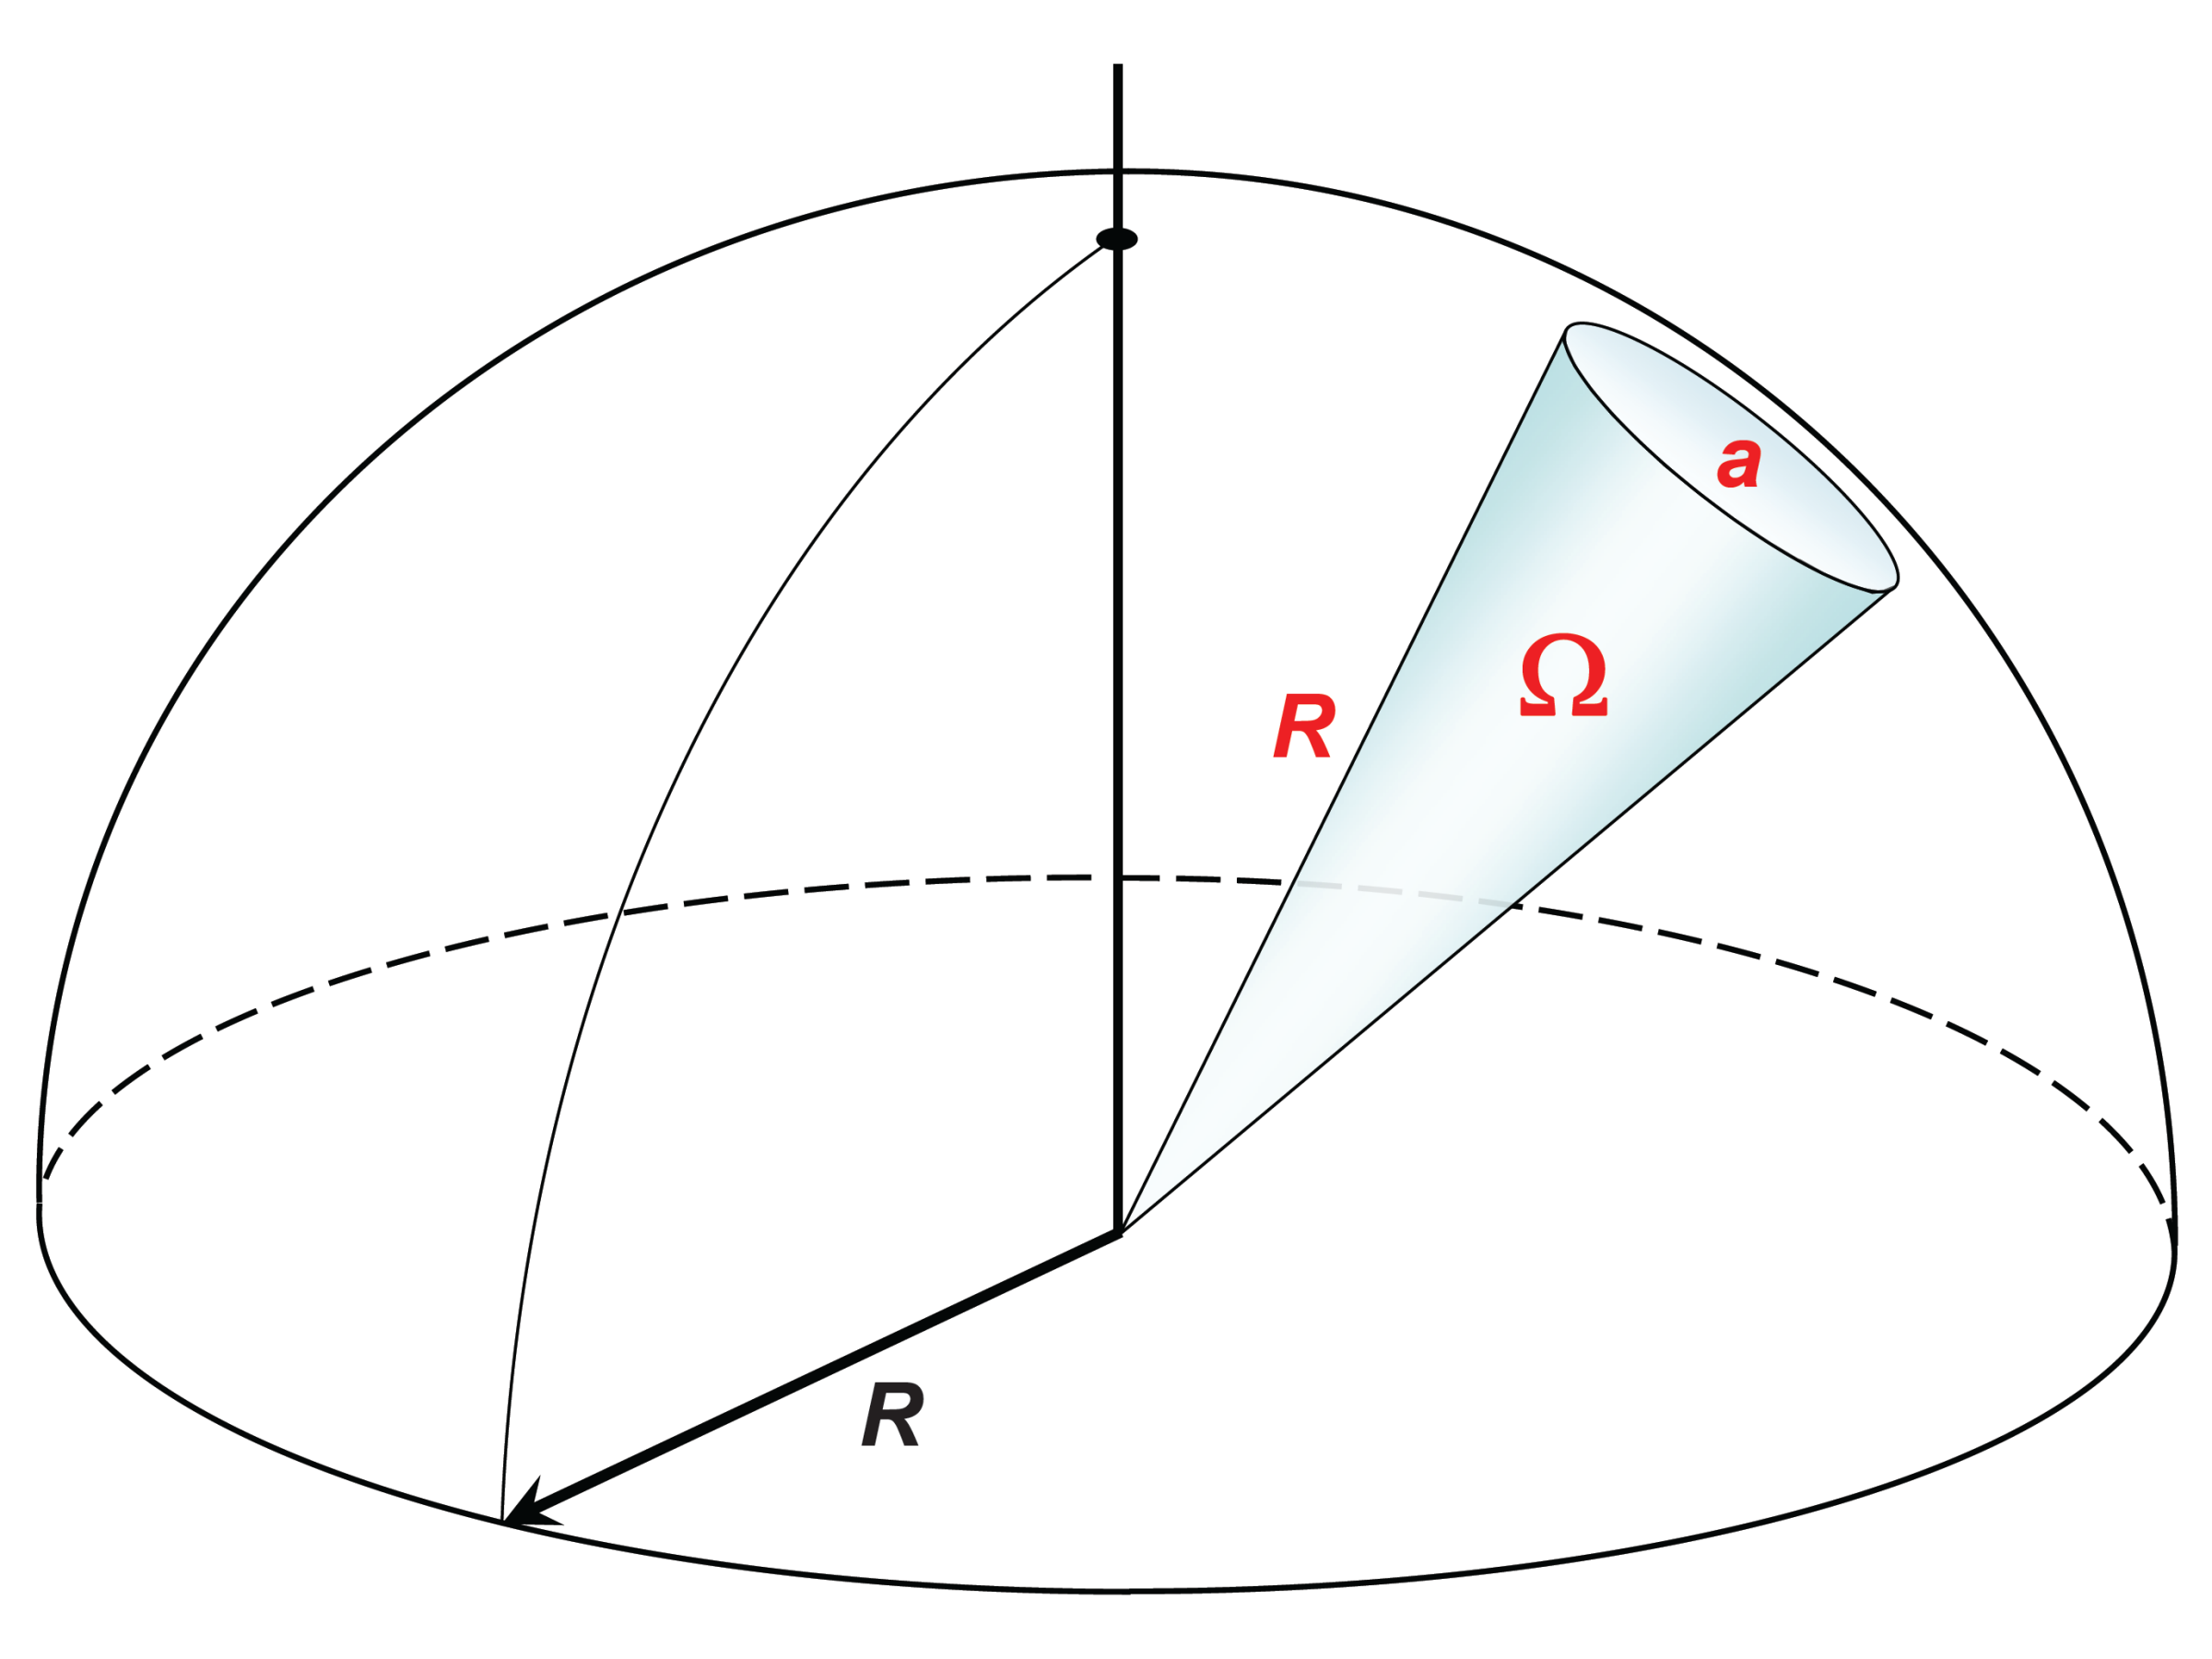
\includegraphics[scale=0.07]{images/solidangle.png}
%   \setcaptioncitation{https://socratic.org/questions/how-much-of-the-total-energy-that-leaves-the-sun-makes-it-to-earth-why}
  \caption{A depiction of the steradian, $\Omega$ of a conic surface area located on a sphere of radius $R$.}
  \label{solid_ang}
\end{figure}

We will get a steradian value for our setup by comparing angular separations to pixel distances in our camera images.
To expand on this, as the Moon travels through the night's sky, it changes locations on our observable hemisphere.
Differences in location on the hemisphere can be described by the angle they form with respect to the observer, the angular separation.
If it were to travel from one horizon directly through the zenith to the other horizon, it would have traveled an angular separation of $180 \deg$.  
If we know the angular separation traveled and the total number of pixels traversed, we can establish a relationship between the two and get a precise steradian value.
Plugging this value into Equation~\ref{area_eq} yields the area of sky observed.
Equation~\ref{area_eq} does well to describe a purely conic field of view.
As we will see see in our methods section, it is also useful to know the area of a rectangular pyramid.
Specifically, we want to know the surface area of a rectangular pyramid's base that has been projected to have a constant radius. 
This resulting area appears as a curved surface that could be imagined as a small square cutout of a sphere.
We see in Figure~\ref{useful_area_equation} a depiction of this shape as well as some equations that help calculate the base's surface area.
With respect to the two angles $a$ and $b$ that determine the size of the base, we find that:

\begin{equation}
\Omega =  4 \arcsin{(\sin{(\frac{a}{2})}\sin{(\frac{b}{2})})}
\label{steradian1}
\end{equation}

where $\Omega$ is the shape's steradian.  
The steradian can be further used to help find the area of the base via the formula:
\begin{equation}
\Omega = \frac{A}{r^2}
\label{steradian1}
\end{equation}
where $r$ represents the distance to the area of the sky you are observing.
Using basic substitution and algebra, we find that the resulting equation for the area of the base in terms of the distance $r$ and the two angles $a$ and $b$ is:

\begin{equation}
A =  4 \arcsin{(\sin{(\frac{a}{2})}\sin{(\frac{b}{2})})} r^2
\label{small_area_eq}
\end{equation}

where $r$ represents the distance to the area of the sky you are observing.
We will see this equation applied in the methods section when converting angular measurements to kilometer measurements.

One might naively assume that the total observation area would remain consistent each night.
However, one must consider clouds and fog when calculating the overall sky area coverage.
This consideration will be dealt with in our secondary analysis and is further discussed in the methods section.


\begin{figure}[ht!]
  \centering
  \includegraphics[scale=0.4]{images/rectangular_pyramid.png}
  \caption[A visual depiction of the surface area of the base of a fixed radius rectangular pyramid, marked $A$, alongside supporting equations.]{A visual depiction of the surface area of the base of a fixed radius rectangular pyramid, marked $A$, alongside supporting equations.  The steradian $\Omega$ is not marked on the leftmost figure because it represents an angle not visible and should not be confused with angles $a$ or $b$.}
  \label{useful_area_equation}
\end{figure}


